\documentclass[final,1p,times]{elsarticle}
%DIF LATEXDIFF DIFFERENCE FILE
%DIF DEL old.tex   Sat Oct 31 16:31:55 2015
%DIF ADD new.tex   Sat Oct 31 16:31:43 2015

%% Use the option review to obtain double line spacing
%% \documentclass[preprint,review,12pt]{elsarticle}

%% Use the options 1p,twocolumn; 3p; 3p,twocolumn; 5p; or 5p,twocolumn
%% for a journal layout:
%% \documentclass[final,1p,times]{elsarticle}
%% \documentclass[final,1p,times,twocolumn]{elsarticle}
%% \documentclass[final,3p,times]{elsarticle}
%% \documentclass[final,3p,times,twocolumn]{elsarticle}
%% \documentclass[final,5p,times]{elsarticle}
%% \documentclass[final,5p,times,twocolumn]{elsarticle}

%% if you use PostScript figures in your article
%% use the graphics package for simple commands
%% \usepackage{graphics}
%% or use the graphicx package for more complicated commands
\usepackage{graphicx}
%% or use the epsfig package if you prefer to use the old commands
%% \usepackage{epsfig}

%% The amssymb package provides various useful mathematical symbols
\usepackage{amssymb}
%% The amsthm package provides extended theorem environments
%% \usepackage{amsthm}
%% algorithms
\usepackage{algpseudocode}
\usepackage{algorithm}
%DIF 30a30
\usepackage{url}
 %DIF > 
%DIF -------

%% The lineno packages adds line numbers. Start line numbering with
%% \begin{linenumbers}, end it with \end{linenumbers}. Or switch it on
%% for the whole article with \linenumbers after \end{frontmatter}.
%% \usepackage{lineno}

%% natbib.sty is loaded by default. However, natbib options can be
%% provided with \biboptions{...} command. Following options are
%% valid:

%%   round  -  round parentheses are used (default)
%%   square -  square brackets are used   [option]
%%   curly  -  curly braces are used      {option}
%%   angle  -  angle brackets are used    <option>
%%   semicolon  -  multiple citations separated by semi-colon
%%   colon  - same as semicolon, an earlier confusion
%%   comma  -  separated by comma
%%   numbers-  selects numerical citations
%%   super  -  numerical citations as superscripts
%%   sort   -  sorts multiple citations according to order in ref. list
%%   sort&compress   -  like sort, but also compresses numerical citations
%%   compress - compresses without sorting
%%
%% \biboptions{comma,round}

% \biboptions{}


\journal{Parallel Computing}

%DIF PREAMBLE EXTENSION ADDED BY LATEXDIFF
%DIF UNDERLINE PREAMBLE %DIF PREAMBLE
\RequirePackage[normalem]{ulem} %DIF PREAMBLE
\RequirePackage{color}\definecolor{RED}{rgb}{1,0,0}\definecolor{BLUE}{rgb}{0,0,1} %DIF PREAMBLE
\providecommand{\DIFadd}[1]{{\protect\color{blue}\uwave{#1}}} %DIF PREAMBLE
\providecommand{\DIFdel}[1]{{\protect\color{red}\sout{#1}}}                      %DIF PREAMBLE
%DIF SAFE PREAMBLE %DIF PREAMBLE
\providecommand{\DIFaddbegin}{} %DIF PREAMBLE
\providecommand{\DIFaddend}{} %DIF PREAMBLE
\providecommand{\DIFdelbegin}{} %DIF PREAMBLE
\providecommand{\DIFdelend}{} %DIF PREAMBLE
%DIF FLOATSAFE PREAMBLE %DIF PREAMBLE
\providecommand{\DIFaddFL}[1]{\DIFadd{#1}} %DIF PREAMBLE
\providecommand{\DIFdelFL}[1]{\DIFdel{#1}} %DIF PREAMBLE
\providecommand{\DIFaddbeginFL}{} %DIF PREAMBLE
\providecommand{\DIFaddendFL}{} %DIF PREAMBLE
\providecommand{\DIFdelbeginFL}{} %DIF PREAMBLE
\providecommand{\DIFdelendFL}{} %DIF PREAMBLE
%DIF END PREAMBLE EXTENSION ADDED BY LATEXDIFF

\begin{document}

\begin{frontmatter}

%% Title, authors and addresses

%% use the tnoteref command within \title for footnotes;
%% use the tnotetext command for the associated footnote;
%% use the fnref command within \author or \address for footnotes;
%% use the fntext command for the associated footnote;
%% use the corref command within \author for corresponding author footnotes;
%% use the cortext command for the associated footnote;
%% use the ead command for the email address,
%% and the form \ead[url] for the home page:
%%
%% \title{Title\tnoteref{label1}}
%% \tnotetext[label1]{}
%% \author{Name\corref{cor1}\fnref{label2}}
%% \ead{email address}
%% \ead[url]{home page}
%% \fntext[label2]{}
%% \cortext[cor1]{}
%% \address{Address\fnref{label3}}
%% \fntext[label3]{}

\title{Hybrid MPI-thread Parallelization of Adaptive Mesh Operations}

%% use optional labels to link authors explicitly to addresses:
%% \author[label1,label2]{<author name>}
%% \address[label1]{<address>}
%% \address[label2]{<address>}

\author[a]{Dan Ibanez\corref{b}}
\ead{ibaned@rpi.edu}
\ead[url]{http://scorec.rpi.edu/~dibanez}
\author[a]{Ian Dunn}
\ead{dunni@rpi.edu}
\author[a]{Mark S Shephard}
\ead{shephard@rpi.edu}

\address[a]{
Scientific Computation Research Center,
Rensselaer Polytechnic Institute,
110 Eighth Street, Troy, NY 12180, USA
}
\cortext[b]{Corresponding author}

\begin{abstract}
%% Text of abstract

Many of the world's leading supercomputer architectures
are a hybrid of shared memory and network-distributed memory.
Such an architecture lends itself to a hybrid MPI-thread programming
model.
We first present an implementation of inter-thread message passing
based on the MPI and pthread libraries.
In addition, \DIFaddbegin \DIFadd{we present }\DIFaddend an efficient implementation of termination
detection for communication rounds\DIFdelbegin \DIFdel{is presented called }\DIFdelend \DIFaddbegin \DIFadd{.
We use the term }\DIFaddend phased message passing \DIFaddbegin \DIFadd{to denote the communication
interface based on this termination detection}\DIFaddend .
This interface is then used to implement parallel operations
for adaptive unstructured meshes, and the performance of resulting
applications is compared to pure MPI operation.
We also present new workflows enabled by the ability to vary
the number of threads during runtime.

\end{abstract}

\begin{keyword}
%% keywords here, in the form: keyword \sep keyword
Hybrid system \sep Shared memory \sep Parallel programming models \sep MPI \sep
Termination detection \sep Non-blocking

%% MSC codes here, in the form: \MSC code \sep code
%% or \MSC[2008] code \sep code (2000 is the default)

\end{keyword}

\end{frontmatter}

%%
%% Start line numbering here if you want
%%
% \linenumbers

%% main text
\section{Introduction}
\label{sec:intro}

The ability to advance parallel processing in an energy efficient
manner requires the continued addition of layers to the hardware
hierarchies.
A key addition that is being shared by all new
HPC hardware is a hybrid model combining the benefits
of closely packed cores with the benefits of distributed memory
by networking together a set of nodes, each of which contains
many cores which share in-node RAM.

Operating systems have the analogous concepts of processes,
which have unique address spaces and executions, and threads, which
have unique executions but shared address spaces.
Each process is a thread since it executes, but more
threads may be created within a process.
All threads in a process share the process' address space.
Taking effective advantage of this hybrid software model is essential
to scalability and parallel efficiency.
However, doing that while not requiring substantial refactoring
of large, complex simulation software requires the insertion
of a new interface that directly replaces the inter-process communication
currently being used by that software.

It is most natural to take advantage of this hardware
configuration by writing programs that map processes to nodes
and threads to cores.
Of course, performance optimization may dictate that certain
ratios of processes to nodes and thread to cores is are more optimal,
but the general idea remains the same.

\DIFdelbegin \DIFdel{Since,
for our purposes, a processis a special
case of a thread, we use }\DIFdelend \DIFaddbegin \DIFadd{All operating system processes start with at least one thread,
sometimes called the master thread.
Extra threads may be created within a process.
Unless otherwise specified, }\DIFaddend the term ``thread" \DIFdelbegin \DIFdel{throughout
to mean either a }\DIFdelend \DIFaddbegin \DIFadd{for the remainder of
this paper denotes an execution instance that can communicate
with others, even in the case when it is just the master
thread of a normal }\DIFaddend process with no \DIFdelbegin \DIFdel{threads or a thread
within a process, and specify the distinction where necessary}\DIFdelend \DIFaddbegin \DIFadd{extra threads}\DIFaddend .

We present here a refinement of the above approach with additional
motivations from a software engineering standpoint.
The MPI programming model has been successful in large part due
to its elegant concept of communicating parallel processes,
and the fact that the hardware actually is composed of communicating parallel
nodes, so the abstraction does not introduce excessive overhead.
This programming model has formed the basis not only for source code
but also the design of scalable algorithms.

Past work has taken the approach of programming two levels of
parallelism, one based on communication and another tailored to shared memory.
Given the established body of algorithms and source code based on the MPI model
and the inherent complexity of using two distinct programming models,
a goal of our work is to preserve this single programming model while enabling
operation which is hybrid at an operating system and hardware level.

This means providing inter-thread communication capabilities equivalent to
those required by existing MPI programs, such that an MPI-based
code can be ported to hybrid operation with essentially no modification.
Note that, since the on-node performance of a hybrid system is better
than its inter-node performance, developers will want want to modify
software to take advantage of shared memory and other locality.
However, such modification can now happen more gradually after the initial
port, and at a higher level than the detailed thread management.

Section \ref{sec:thread} introduces the standard support for
threading and communication on which this work is built, and Section
\ref{sec:related} gives an overview of related hybrid systems also
built on this support.
Section \ref{sec:p2p} details the implementation of inter-thread message
passing at the heart of our system, and Section \ref{sec:coll} covers
collective operations.
The phased algorithm for termination detection is derived in Section
\ref{sec:phased}, which proves useful to unstructured applications
regardless of threading model.

These combined capabilities
are packaged into a C library called the Parallel Control Utility\DIFdelbegin \DIFdel{, or PCU }\DIFdelend \DIFaddbegin \DIFadd{.
PCU is available under the BSD 3-clause license for researchers interested
in its source code: }\url{https://github.com/SCOREC/core/tree/master/pcu}\DIFaddend .
This library is used to implement a variety of adaptive unstructured
mesh operations, which enables them to execute in a hybrid environment.
Two specific operations serve as illustrative examples:
mesh migration in Section \ref{sec:migrate} and repartitioning in
Section \ref{sec:repart}.
The performance of these mesh operations is presented and discussed in
Section \ref{sec:results}.

\section{Supporting Technology}
\label{sec:thread}

There are several layers of support built into the system software 
of HPC architectures on which the parallel control utility
presented in this paper relies.
Our primary target architectures are
HPC systems consisting of a large number of distributed memory nodes
where each node has a large number of cores sharing common memory.
Current testing is done on the IBM Blue Gene/Q, although
the design has been kept general enough that our system runs
on other targets such as the Intel Xeon Phi.

There are two dominant thread management interfaces, pthreads and OpenMP.
The pthreads library is more general, standard, and can directly create
and destroy single threads.
OpenMP focuses on HPC-style thread parallelism and ease of use,
\DIFdelbegin \DIFdel{with the model of an unaltered thread pool
which supports user tasks
}\DIFdelend \DIFaddbegin \DIFadd{allowing users to execute tasks in a batched fork-join style,
which may be implemented underneath using a thread pool
}\DIFaddend \cite{dagum1998openmp}.
In our work, we adopt \DIFdelbegin \DIFdel{the same thread pool model as }\DIFdelend \DIFaddbegin \DIFadd{a similar model to }\DIFaddend OpenMP but
maintain control of the threads through pthreads.
This should allow us to integrate with OpenMP-based codes
in the future, by using OpenMP's C function interface.

The other system library of importance is MPI.
The MPI standard has introduced a multi-level system of thread safety.
That is to say that the MPI library will perform correctly when
interacted with by multiple threads per process, but it
continues to think in terms of inter-process communication.
For initial simplicity, our code uses the MPI\_THREAD\_MULTIPLE
level of support, but we could adjust down to MPI\_THREAD\_FUNNELED
without much difficulty \cite{balaji2008toward}.
There are issues involved with the implementation of a thread-safe
MPI library \cite{gropp2006issues}, and even a testing framework
developed to measure the ability of an MPI implementation
to support such use \cite{thakur2007test}.
These are performance concerns that can be addressed by moving
more of the synchronization responsibility to our user-level code.

The Blue Gene/Q has a few restrictions which are naturally resolved
through the use of threads.
First, individual process creation by the user is not possible, so
changing the degree of parallelism (number of running threads)
is only possible by creating threads in processes.
Second, the executable instructions for a user's program and its
required libraries are loaded into system memory once for each process.
By using less processes with multiple threads per process, one gets
an equal level of parallelism with reduced memory use by executable
instructions.
This principle also applies to program structures which are allocated
once per process, such as those of the MPI library.

Finally, the MPI implementation on the Blue Gene/Q is configured to
create its own helper threads on unused cores to help improve
the performance of user programs which do not create threads.
However, one should disable this feature in order to free the cores for
user-created threads.

\section{Related Work}
\label{sec:related}

The study of hybrid MPI and threads is receiving serious attention
at the time of this writing, as are parallel mesh-based simulation
methods.

Mavriplis studied the performance of an unstructured mesh
Navier-Stokes solver using MPI and OpenMP, as well as the same
scheme for using MPI to send messages between threads that
we employ in Section \ref{sec:p2p}.
He found significant speedup when using a two-level message
passing scheme instead, with 140 processes on an SGI-Origin 2000
\cite{mavriplis2002parallel}.

On the Blue Gene/Q, Kumar et al. developed a series of fine-grained
threading techniques in concert with Charm++ and achieved good
scaling of the NAMD molecular dynamics code using high thread
per process counts on several hundred thousand cores
\cite{kumar2013acceleration}.

Cramer et al. have studied the use of OpenMP on the Intel Xeon Phi
chip and show that CPU-targeted code can be ported to it fairly
easily with decent speedup \cite{cramer2012openmp}.
Dokulil et al. created a C++ system for array-based operations
which runs in hybrid on the host and Phi co-processor and distributes
work based on a parallel-for paradigm \cite{Dokulil20132508}.

In general, mesh-based simulation methods have entered the billion element,
billion degree of freedom era.
With such large meshes, there are only a few machines capable of running
these simulations.
Komatitsch et al. use a Spectral Element Method for earthquake simulation
that reaches 14.6 billion degrees of freedom.
Running on the Earth Simulator machine, it simulates earthquake propagation
over the entire planet \cite{komatitsch200314}.
Stowell et al. simulate radar wave propagation through buildings using
a 10 billion element regular Cartesian grid mesh
\cite{stowell2008investigation},
and Burstedde et al. use adaptive mesh refinement to create a
12.4 billion element mesh for mantle convection simulations
on TACC's Ranger computer \cite{burstedde2008scalable}.
Rasquin et al. \cite{rasquin2014scalable} simulate the influence of active flow control
devices on airfoil drag reduction with meshes of 92 billion elements
running on the Mira Blue Gene/Q at Argonne National Laboratory.

\section{Inter-thread Message Passing}
\label{sec:p2p}

The main unusual design choice of PCU compared to
other hybrid programming systems is
its focus on inter-thread message passing.
Since we must rebuild some of the high-level message
passing capabilities, we identify a set of primitive
operations as described by the MPI standard \cite{walker1996mpi}
which are sufficient for our applications:

\begin{enumerate}
\item Non-blocking synchronous send
\item Non-blocking send request completion test
\item Non-blocking probe
\item Blocking receive
\end{enumerate}

These conceptual message-passing primitives are independent
of their particular implementation.
Note that because we require the send operation to be synchronous,
it will complete if and only if the message is completely received at its
destination.

All the remaining algorithms rely only on these guaranteed properties
of the message passing primitives.
To develop inter-thread message passing, we implement inter-thread
message passing passing primitives.
These are currently based on calling thread-safe MPI versions of the
same primitives, but an area of future work involves implementing
more efficient primitives.

In order to use MPI itself to pass messages between threads, we require
that the implementation correctly handle self-sends.
Then, we need to encode the source and destination thread IDs into the message
metadata such that messages can be multiplexed out of a single process
and demultiplexed at their destination process.
The encoding of thread IDs makes use of the standard MPI\_TAG metadata
integer, which is typically a 32-bit signed integer.
We use 10 bits of this integer to encode each of the local IDs for the
source and destination threads.
This encoding of source and destination means that threads must inspect
messages with more sophisticated checking of the tag than MPI\_RECV
offers, since messages arriving at the same process may be destined
for different threads within that process.
We use MPI\_IPROBE to inspect the tag before using MPI\_RECV to commit
to being the receiver.
This combined probe and conditional receive procedure is specified
in Algorithm \ref{alg:receive}.

\begin{algorithm}
\caption{Non-blocking pattern-match receive}
\label{alg:receive}
\begin{algorithmic}
\Function{receive}{pattern $P$}
\State let message $M \gets$ non-blocking probe
\If{$M$ is null (there is no message)}
\State \Return null
\EndIf
\If{metadata of $M$ does not match $P$}
\State \Return null
\EndIf
\State allocate buffer $b$ per metadata of $M$
\State blocking receive $M$ into $b$
\State \Return $(M,b)$
\EndFunction
\end{algorithmic}
\end{algorithm}

\section{Non-Blocking Collectives}
\label{sec:coll}
Collective operations are a necessary staple of
distributed-memory high-performance computing.
Operations such as parallel reduction, broadcast, and other collectives
are key to coordinating threads \cite{pjevsivac2007performance}.
More details on these collective algorithms and tradeoffs in their
implementation can be found in \cite{thakur2003improving}.
Non-blocking collectives are more advanced implementations which
are typically used to overlap communication and computation.
By using them, PCU benefits from this overlap.
Furthermore, in Section \ref{sec:phased}, we present an algorithm
for which blocking collectives are insufficient, and a non-blocking
implementation is not just convenient but necessary.

Since collectives are used by nearly all applications,
we place a focus on developing built-in
multithreaded collective operations based on the
inter-thread message passing primitives.

We consider three fundamental collective operations:
broadcast, reduce, and scan.
Other operations such as exclusive scan and all-reduce
can be built from the first three.
These operations were selected as the minimal subset
of collectives needed for our unstructured mesh operations.

These three collectives share many common features:
they use $O(\log n)$ steps for $n$ threads,
and at each step each thread is either idle, sending one
message, or receiving one message.
These shared characteristics make it easier to implement
all the collectives in a general framework which abstracts
away their differences, starting with the specific communication
pattern used.
A thread only needs to know which of the three actions to perform at each
step and with which thread it is communicating, if any.
This combined information is referred to as the communication pattern.

The second abstraction we can make is that of a merge operator, which is
essentially the MPI reduction operator (e.g. MPI\_SUM or MPI\_MAX).
The merge operator modifies the local data based on incoming data.
For example, an reduction sum adds incoming values to local values.
We do not refer to it as the reduction operator because it is used
in all cases, including broadcast.
As an interesting corner case, the merge operator for broadcast simply
assigns the incoming value as the local value.

Following good software design, the communication pattern,
merge operator, and data are each specified separately
and are orthogonal from one another.
This follows the example of interfaces such as MPI\_REDUCE.

With these abstract components specified, we can execute a collective
operation
using the non-blocking point-to-point message passing primitives
developed in Section \ref{sec:p2p}.
Although the simplicity of collectives would allow blocking primitives
to be used, using non-blocking primitives gives us a great benefit:
we obtain a non-blocking collective operation.
Such operations have been implemented before \cite{hoefler2007implementation}
and subsequently proposed for the latest MPI standard \cite{hoefler2006non}.
Our work implements hybrid threaded versions of such collectives.

Users of this system initiate a collective operation, and can interleave
computation with communication progress queries.
Communication progress consists of checking for incoming messages in the current
step and proceeding to the next step when they are received.

Non-blocking collectives are useful from the perspective of
of hiding latency, but they will prove to be indispensable to
Algorithm \ref{alg:phased}.

\section{Phased Message Passing}
\label{sec:phased}

A common problem that arises when dealing with parallel graphs,
and similar structures, such as the adjacency relations of unstructured
meshes, has to do with transporting graph, or mesh entities, from
one thread to another
due to changes in the graph or to other operations which affect
load balance.
Such transportation is specified in a one-sided,
push-driven manner, which means that each thread knows which
entities it should send to which other threads, but does
not know what it will be receiving.

Without {\it a priori} knowledge of the extent of information to be
received, it is difficult to determine when to stop receiving
information.
A thread can perform a continuous loop which receives messages,
but we must determine when to terminate that loop.

This problem has been solved previously in a slightly less efficient
manner \cite{Ovcharenko2012140}, and is an important special case
of the general termination detection problem.
Here we present an optimal solution based on non-blocking barriers.
The fundamental idea is this: all threads can stop receiving
once all messages have been received.
Given an individual message, we can use the synchronous non-blocking
send provided by MPI to inform the sending thread of when the message
is fully received by the receiving thread.
In this way, each thread can be informed upon the successful receipt
of each message it sends.

If each thread keeps track of these send completions then,
at some point, each individual thread is aware that every
messages it sent has been received.
If all threads could synchronize after that event, then
we would know that all messages are received.
Synchronizing after an event is usually done with a barrier,
however in this case there is a problem with using a blocking barrier.
If a thread enters a blocking barrier after messages it sent
have been received, it may indefinitely ignore incoming messages
which it is still responsible for receiving.
In other words, the thread is done sending but it is not done receiving.
This means that threads must continue to accept messages until
the barrier is over, which necessitates a non-blocking barrier.
The operation of sending and receiving messages this way
is here referred to as a communication phase.
The procedure for a single communication phase is more precisely defined
by Algorithm \ref{alg:phased}.

\begin{algorithm}
\caption{Phased message passing}
\label{alg:phased}
\begin{algorithmic}[1]
\Function{phase}{outgoing messages $M$}
\State let $R \gets$ the requests from synchronous non-blocking sends of $M$
\While{there are incomplete requests in $R$}
\State receive and process messages
\EndWhile
\State begin non-blocking barrier
\While{non-blocking barrier is not done}
\State receive and process messages
\EndWhile
\EndFunction
\end{algorithmic}
\end{algorithm}

The runtime properties and bounds of Algorithm \ref{alg:phased} are vital
to the scalability of user applications.
As such, we will derive the important runtime properties and show how
they are optimal in terms of the target applications.

Given a set of messages $M$, the time required to fully transmit them
can be approximated as $O(\alpha|M| + \beta\|M\|)$, where
$|M|$ is the number messages and $\|M\|$ is the total sum of their
content sizes, while $\alpha$ and $\beta$ are arbitrary constants
representing latency and inverse bandwidth, respectively.

Let us examine the runtime of Algorithm \ref{sec:phased} line-by-line.
The runtime of line 2 is simply $O(|M|)$ since sends are non-blocking.
The time for the loop on lines 3-5 is the time it takes
for sends of $M$ to be acknowledged, which is on the same order
as the time required to transmit $M$ since each message just incurs
constant added latency waiting for acknowledgement.
The loop on lines 7-9 is bounded by the maximum of barrier and receive times.
Our non-blocking barrier is implemented using an $O(\log n)$ algorithm where
$n$ is the total number of threads.
The worst case for receive time is if all incoming messages get received at
line 8.
Let $I$ be the set of incoming messages, then given linear-time processing
the second loop requires at least time $O(\beta\|I\|)$.
We will omit latency costs for $I$ since the thread is only receiving
and it will not alter our conclusions.
In total, the communication phase requires time on the order of:

\[O(\alpha|M| + \beta\|M\| + \max(\beta\|I\|,\log n))\]

In our use cases, $|M|$, $\|M\|$ and $\|I\|$ are
not dependent on the number of threads $n$ so, with respect to $n$,
a communication phase is essentially bound by the barrier's $O(\log n)$ time.
Note that we do overlap all incoming message processing with all outgoing
message wait operations, so the potential for latency hiding is maximized.

When implementing phased message passing, we also optimize performance
by buffering messages.
The user interface of phased communication allows us to pack
all data traveling between the same pair of threads into a single message.
This is done prior to executing Algorithm \ref{alg:phased}.
As such, the number of messages sent $|M|$ is equal to the number of unique
destinations and the number of messages received $|I|$ is equal to the number
of unique sources.

This relation of message counts to communication neighbors (sources and
destinations) is quite useful in the process of determining runtime bounds.
This is because, due to mesh partitioning, each thread has a small
and constant number of neighbors,
about 40 at most \cite{zhou2010petascale}.
This limits the source and destination counts to 40 as well.

We have shown previously that this buffering can greatly improve performance
due to the latency cost $\alpha$ and MPI's own management overhead per message,
especially for applications
with a tendency to send very small messages between the same pair of threads
\cite{Ovcharenko2012140}.
In the case of multiple threads per process, buffering also reduces
the number of calls to MPI\_SEND and MPI\_RECV, which reduces
contention for the MPI library between the threads in that process.
When these calls are protected by a lock, avoiding contention is important
\cite{mavriplis2002parallel}.

\section{Migration Use Case}
\label{sec:migrate}

We now move to describing the application of PCU to massively parallel
adaptive finite element simulations.
Such simulations make use of unstructured meshes which are
being adapted as the simulation is run on a supercomputer 
\cite{Gal10,rasquin2014scalable,Zhou-flow}.
The mesh is partitioned, giving a subset of its elements to each thread 
\cite{rasquin2014scalable,zhou2012unstructured,Zhou-ewc}.

There are many situations in which we would like to change the partitioning,
i.e. move elements from one thread to another.
This operation, called mesh migration \cite{seol06,shephard2010flexible,Zhou-ewc}, 
arises in many scenarios. When described in terms of threads, this 
operation includes the following types of operations:
\begin{enumerate}
\item Changes in the number of elements per thread that must be
rebalanced.
\item Threads requiring data from elements on another thread. 
\item New threads being created and existing elements moved onto them
\end{enumerate}
Since only the thread which has a particular element knows the full details of
the element, threads performing migration
typically know only which of their own elements will be sent to other threads,
but not which elements they will receive.
This is exactly the communication problem described in Section \ref{sec:phased},
and thus migration is a primary motivator of the phased communication
algorithm.

Although the migration algorithm is fairly complex, we can give a simplified
definition to illustrate the use of PCU.
A detailed description of migration can be found in \cite{seol06,shephard2010flexible}.
Each mesh entity (vertices, edges, triangles, and tetrahedra) is an object with
adjacency relations to objects of lower dimension, as well as relations
to copies representing the same entity on another thread.
A pre-processing stage of migration determines, for each entity, the set of
threads to which new copies must be sent.
One of the existing copies is designated as the ``original" copy from which
new copies are made.
To reconstruct the mesh on the receiving end, we send entities in order of
increasing dimensionality.
This ensures new vertices exist when new edges are being constructed, etc.
Finally, the remote copy relations must be updated by echoing newly
created copies back to the original to collect the new set of remote copies.

These processes are outlined in Algorithm \ref{alg:send}.
Per the notation in \cite{shephard2010flexible}, $\{M_o^d\{M^{d-1}\}\}$ denotes
the set of entities of dimension $(d-1)$ adjacent to entity $M_o^d$ of dimension $(d)$.

\begin{algorithm}[!ht]
\caption{Send entities}
\label{alg:send}
\begin{algorithmic}[1]
\Function{send\_entities}{mesh $M$}
  \For{dimension $d$ from 0 to 3}
    \For{original copy $M_o^d$}
      \State let $A \gets \{M_o^d\{M^{d-1}\}\}$
      \For{thread $t$ to which $M_o^d$ must be sent}
        \State let $A_R$ be the copies of $A$ on $t$
        \State pack $(M_o^d,A_R)$ in message to $t$
      \EndFor
    \EndFor
    \State begin communication phase 1
    \For{$(M_o^d,A_R)$ received from $t$}
      \State construct $M_n^d$ from $A_R$
      \State pack $(M_o^d,M_n^d)$ in message to $t$
    \EndFor
    \State begin communication phase 2
    \For{$(M_o^d,M_n^d)$ received from $t$}
      \State record $M_n^d$ as a remote copy of $M_o^d$
    \EndFor
  \EndFor
\EndFunction
\end{algorithmic}
\end{algorithm}

At the beginning of a communication phase, all messages which have been packed
up to that point are sent and cleared.
During a phase, messages which were sent at the beginning of that
phase are received.

The reason that we do not denote a communication phase with a simple
call has to do with the non-blocking nature of the phased message passing
algorithm.
In the for loop given in lines 11-14 of Algorithm \ref{alg:send}, the program is simultaneously
receiving and processing messages from phase 1,
while the termination detection for phase 1 is running.
The loop will terminate when the phased algorithm terminates.
Part of the message processing, in this case, involves creating 
content to send in phase 2.
The conditions are similar in lines 16-18 in which the loop will terminate
when phased message passing detects that there are no messages to receive.
In this case, there are no more phases to pack for.

At the end of this algorithm, all new copies have been created with
the mesh adjacency relations fully updated  \cite{seol06,shephard2010flexible} 
and the original copies have a full list
of all the newly created copies.
This is accomplished with only two non-blocking barriers in the background even though
threads could not anticipate the sources or lengths of incoming messages.

This background synchronization sits in contrast to synchronization
schemes in which all threads are blocked during a barrier.
Using PCU, these threads are constantly doing important user-level work,
and will only be blocked by the barrier if the amount of user work
to do in one phase is faster to complete than the barrier itself.

\section{Threaded Repartitioning}
\label{sec:repart}

Ideally, an adaptive finite element simulation would run once on a large supercomputer,
accepting a problem description and automatically generating a mesh in parallel, 
and entering a parallel loop that that iteratively solves the PDEs on that mesh, estimates the
discretization errors and improves the mesh until the desired level
of solution accuracy is obtained \cite{Gal10,rasquin2014scalable,Zhou-flow}.
However, the relative scalability of the different steps, the fact that the problem size is 
changing as the simulation continues coupled with the fact that the queuing and operating 
systems of massively parallel computers does not support the automatic changing of number
of cores assigned during a run, motivates an incremental approach, in which
a coarse initial mesh is generated using a small number of cores and is scaled
up using successively larger machine allocations as the mesh is adapted \cite{rasquin2014scalable}.

Consider the workflow for the simple case of first generating a ``coarse" mesh
with $N$ parts and $e$ elements,
that is successively refined in a series of $T$ steps using some multiplication factor $m$
such that each step multiplies the number of elements and parts by $m$.
At the end of this process, the mesh has $(em^T)$ elements and $(Nm^T)$ parts.
Increasing element counts is done using mesh refinement, and 
increasing part counts is done using a combination of partitioning tools \cite{rasquin2014scalable}.

Although research is ongoing on choosing combinations of partitioning tools, we
will focus on the following concrete approach, which has been used
successfully to generate meshes of up to 92 billion elements
\cite{rasquin2014scalable,zhou2012unstructured}.
The local graph partitioner used is
the ParMETIS graph partitioner \cite{karypis2011metis},
which is in turn being used through Zoltan\cite{devine2002zoltan}.
The global diffusive repartitioner is ParMA \cite{rasquin2014scalable,zhou2012unstructured}.
The up-scaling workflow proceeds as follows:

\begin{enumerate}
\item An $N$-part mesh is loaded in parallel on $N$ processors
\item Mesh refinement multiplies the element count by $m$
\item A local graph partitioner separates each part into $m$ parts
\item A global diffusive repartitioner further improves balance
\item The resulting $Nm$ parts are output
\end{enumerate}

Because $N$ processors are used, each process must handle its
$m$ output parts serially.
We can improve upon this by using $Nm$ processors as follows:

\begin{enumerate}
\item An $N$-part mesh is loaded in parallel on $N$ of the $Nm$ processors
\item Mesh refinement multiplies the element count by $m$
\item A local graph partitioner separates each part into $m$ parts
\item Migration distributes these parts onto the $Nm$ processors
\item A global diffusive repartitioner further improves balance
\item The resulting $Nm$ parts are output
\end{enumerate}

Now, every step from migration onwards runs with increased parallelism.
Since the parallel mesh algorithms are best written for the case when
the number of threads equals the number of mesh parts, we would prefer
a system that can change the number of threads from $N$ to $Nm$.

The MPI standard defines MPI\_SPAWN, which is a functionality to create
new processes, but machines such as the IBM Blue Gene/Q do not support
user-triggered operating system process creation for efficiency reasons.
On the other hand, they do support user creation of threads within a
process.

We take advantage of this by creating $m$ threads on each of $N$ initial
processes, thereby creating $Nm$ total threads.
PCU's API provides exactly the same message passing capability to these
threads, and the user communication code written using PCU is the same when
operating on $N$ processes or $Nm$ threads.
The migration, diffusive repartitioning, and result output codes were
written using PCU, whose programming model is general enough to support
all these algorithms.

Because the transition from $N$ to $Nm$ threads requires the initial
$N$ threads to send all mesh entities to the other $N(m-1)$ threads,
the maximum speedup for the migration step is 2x since only the
receiving half is parallelized.
However, the subsequent global diffusive repartitioning and 
output steps receive full $Nm$ parallelism.

In addition, due to the lack of MPI\_SPAWN mechanisms, the old approach
required two levels of programming: one to handle inter-processor
communication and one to handle activity between the $m$ parts on
a single process.
This new approach allows all algorithms to be written for the simple
model of one thread per part, and achieves the desirable outcome of increasing
performance while decreasing the size of the source code and
allowing the hardware to maintain its efficient restrictions.

\section{Results and Discussion}
\label{sec:results}

In order to test the capability of the hybrid MPI-thread system, PCU,
a 1.6 billion element mesh is created using up to 16K cores of an
IBM Blue Gene/Q.
We then run several stress tests on the resulting mesh to quantify
the efficiency of hybrid parallelism.

Mesh generation begins with a 4-part, 400K element tetrahedral
mesh and proceeds so as to maintain a part density of 100K elements
per part.
Each up-scaling repartitioning uses uniform mesh refinement, which
multiplies element counts (and thus part counts) by 8.
On the Blue Gene, we use 2 processes per node initially which results
in 16 threads per node or one thread per core at the end.

\begin{figure}[!ht]
\begin{center}
\caption{Times for hybrid up-scaling}
\label{fig:scale}
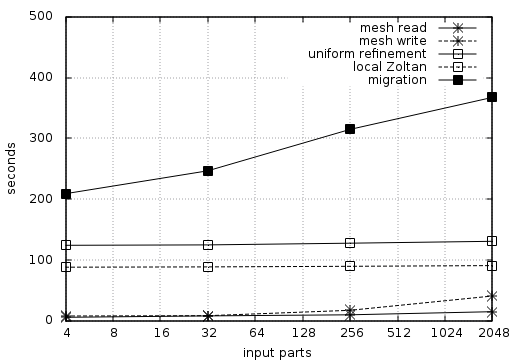
\includegraphics[width=0.7\textwidth]{scaling.png}
\end{center}
\end{figure}

Figure \ref{fig:scale} shows the time consumed by each step of the
PCU supported workflow as the number of parts is increased from 4 to
16K.
The final step converts 2K parts into 16K parts.
In this workflow, migration and mesh file writing is always being
done using 8 threads per process.
By comparison, file reading is done without multithreading,
and the times are very comparable even though each process
is writing 8 times more data, so thread parallelism is achieved.
Migration shows a large increase in runtime as part count is
increased.
This can be explained by Figure \ref{fig:neighbor}, which
shows how the number of neighbor parts to any given part
is increasing at the same rate as the mesh scales up.

\begin{figure}[!ht]
\begin{center}
\caption{Neighborhood increase during up-scaling}
\label{fig:neighbor}
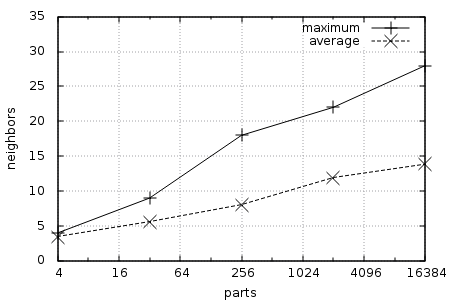
\includegraphics[width=0.6\textwidth]{neighbor.png}
\end{center}
\end{figure}

Recall from Sections \ref{sec:phased} and \ref{sec:migrate} that
phased communication and migration times are directly determined
by neighborhood sizes.
Research shows that there should eventually be a steady-state
neighbor count around 40 \cite{zhou2010petascale}, at which point this
runtime will level off.

In Section \ref{sec:repart}, we predicted a speedup of 2 for
the threaded migration in this workflow compared to its non-threaded
equivalent.
In Figure \ref{fig:repart}, we measure the migration time required
to divide the 2K part, 200 million element mesh by different factors.
The final case results in a 32K part, 200 million element mesh.
As this figure shows, we achieve the maximum predicted speedup.
It is interesting to also note that the threaded version uses
inter-thread message passing while the non-threaded code directly
copies memory.
If the message passing mechanism were significantly slower than
copying, we would have lost much of this speedup.

\begin{figure}[!ht]
\begin{center}
\caption{Threading speedup for repartitioning}
\label{fig:repart}
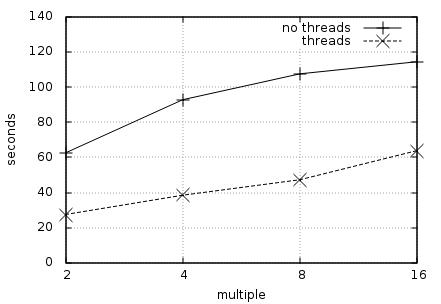
\includegraphics[width=0.6\textwidth]{repart.png}
\end{center}
\end{figure}

Finally, we study the overhead of threading with
a simple workflow.
Beginning with $N$ processes and $m$ threads per process
such that $Nm$ always equals 16K, we read the 16K-part,
1.6 billion element mesh.
In terms of hardware, we are using 16K cores of the Blue Gene/Q,
which is 1024 nodes or one full rack.
Then every thread migrates 10K elements to one of its
neighbors.
The resulting mesh is then written out.
All operations are done in the hybrid mode, and the
number of threads per process $m$ is varied.
In all cases, the ideal outcome is that runtime
remains the same.

\begin{figure}[!ht]
\begin{center}
\caption{Hybrid File IO performance}
\label{fig:fileio}
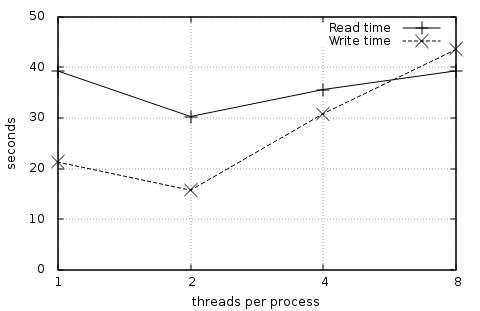
\includegraphics[width=0.6\textwidth]{fileio.png}
\end{center}
\end{figure}

Figure \ref{fig:fileio} shows the times for hybrid file IO.
File IO is more prone to fluctuation because the filesystem
and associated networks are shared by all users.
Despite this, we see file IO performance remains
fairly constant as we move from process-only to hybrid operation.

\begin{figure}[!ht]
\begin{center}
\caption{Hybrid migration performance}
\label{fig:migrate}
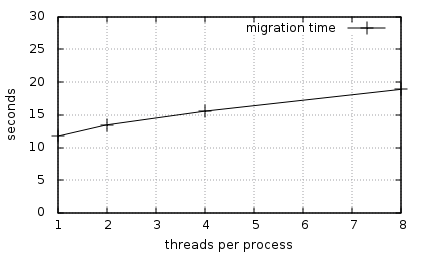
\includegraphics[width=0.6\textwidth]{migrate.png}
\end{center}
\end{figure}

Figure \ref{fig:migrate} shows migration time over threads per process.
Since the ideal result is constant, we see a logarithmic overhead
in this part of the workflow.
This is most likely attributed to having a single MPI instance per process
which must handle the message passing during mutually exclusive calls
by threads \cite{mavriplis2002parallel}.
We intend to explore a custom implementation of inter-thread message passing
in the future to reduce this overhead.

\begin{figure}[!ht]
\begin{center}
\caption{Available memory with threads}
\label{fig:memory}
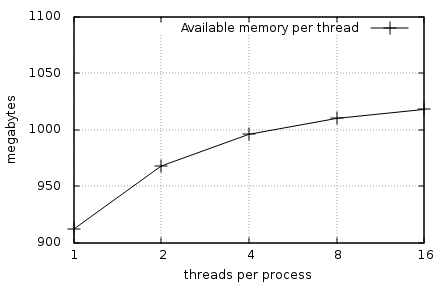
\includegraphics[width=0.6\textwidth]{memory.png}
\end{center}
\end{figure}

As noted in Section \ref{sec:thread}, an important benefit
of threading is to reduce the amount of static memory used, thus increasing
the available memory for user data.
Figure \ref{fig:memory} shows the available memory \emph{per thread} at
each level of threads per process.
The size of the executable used was approximately 90 MB, which was copied
16 times initially.
Using 16 threads, there is now only one copy of the executable and each thread
has about 100 MB of additional free memory due to reduced executable copies
and other static memory allocated per process.
On a machine such as this Blue Gene which allocates about 1 GB to each core,
this is 10 \% of the core's total memory.

\section{Closing Remarks}
\label{sec:conclusion}

We have presented an implementation of non-blocking inter-thread message passing
from which we build non-blocking collectives and the powerful phased
message passing algorithm.
These message passing capabilities are used to implement a variety of
operations for handling adaptive unstructured meshes, and
these operations show good speedup over threads per process.
In addition, the use of threads overcomes certain 
limitations and can lead to greater memory performance than is
attainable through processes alone.

\section*{Acknowledgements}

This work was supported by the Office of Advanced Scientific Computing Research,
Office of Science, U.S. Department of Energy, under grant DE-SC00066117
(FASTMath SciDAC Institute) and in part by the National Science Foundation under
grants OCI-1126125 and IIP-1237555. We gratefully acknowledge the use of the
resources of the Rensselaer Center for Computational Innovations and the
Leadership Computing Facility at Argonne National Laboratory.

%% The Appendices part is started with the command \appendix;
%% appendix sections are then done as normal sections
%% \appendix

%% \section{}
%% \label{}

%% References
%%
%% Following citation commands can be used in the body text:
%% Usage of \cite is as follows:
%%   \cite{key}         ==>>  [#]
%%   \cite[chap. 2]{key} ==>> [#, chap. 2]
%%

%% References with bibTeX database:

\bibliographystyle{elsarticle-num}
\bibliography{ibanez2014}

%% Authors are advised to submit their bibtex database files. They are
%% requested to list a bibtex style file in the manuscript if they do
%% not want to use elsarticle-num.bst.

\end{document}
